\documentclass[border=2mm]{standalone}
\usepackage{amsmath}
\usepackage{tcolorbox}
\usepackage[fontsize=15pt]{fontsize}
% standalone 类通常不需要页眉页脚设置

\usepackage{xeCJK} % 用于处理中文排版
\setCJKmainfont[AutoFakeBold=true]{STKaiti} % 设置中文主字体为华文楷体
\usepackage{fontspec}
% 设置英文主字体为 Times New Roman
\setmainfont{Times New Roman}
\usepackage{graphicx}
% 如果需要使用tikz绘图,取消下面的注释
\usepackage{tikz}
\usetikzlibrary{calc}
\usetikzlibrary{shadings}

% \usetikzlibrary{...}

\begin{document}


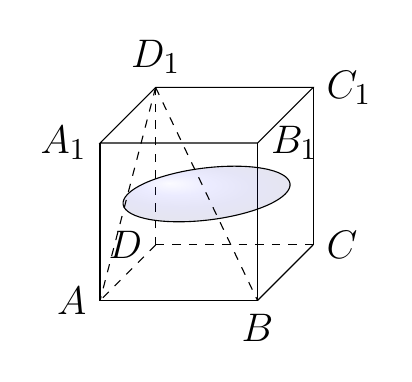
\begin{tikzpicture}[
    y={(0.353cm,0.353cm)},   % 设置 y 轴方向  % 设置 x 轴方向,右手系,y的正方向往里
    x={(1cm,0cm)},           % 设置 x 轴方向
    z={(0cm,1cm)}             % 设置 z 轴方向
]%斜二测画法
% 正方体定义
%-----------------------------------------------------------------------------------------------------------------------
            % 定义矩体的尺寸
            \def\a{2} % 长    
    \begin{scope}

            % 定义顶点
            \coordinate (A) at (0,0,0);
            \coordinate (B) at (\a,0,0);
            \coordinate (C) at (\a,\a,0);
            \coordinate (D) at (0,\a,0);
            %--- 用循环定义顶面端点, A_1,...,D_1
            \foreach \point in {A,B,C,D} {
                \coordinate (\point_1) at ($(\point) + (0,0,\a)$);
            }
            %绘制实线
                %---顶面实线
                \draw (A_1)--(B_1)--(C_1)--(D_1)--cycle; 
                %---和B连接的三条实线
                \foreach \point in {A,B_1,C} {
                    \draw (B)--(\point);
                }
                \draw (A)--(A_1) (C)--(C_1); 
            %绘制虚线
                %---和D连接的三条虚线
                \foreach \point in {A,D_1,C} {
                    \draw[dashed] (D)--(\point);
                }
            % 正方体定点符号
            %-----------------------------------------------------------------------------------------------------------------------
                \node[left] at (A) {$A$};
                \node[below ] at (B) {$B$};
                \node[ right] at (C) {$C$};
                \node[left] at (D) {$D$};
            
                \node[left] at (A_1) {$A_1$};
                \node[right ] at (B_1) {$B_1$};
                \node[ right] at (C_1) {$C_1$};
                \node[above] at (D_1) {$D_1$};
            
    \end{scope}




    \shade[fill opacity=0.1 ,ball color=blue] (\a/2,\a/2,\a/2) circle (\a/2);

    \draw (\a/2,\a/2,\a/2) circle (\a/2);

%填色
% %-----------------------------------------------------------------------------------------------------------------------
%     \begin{scope}
%         \fill[fill opacity=0.1,blue] (A)--(B)--(C)--(D)--cycle;
%         \fill[fill opacity=0.1, red] (A)--(B)--(D_1)--cycle;  
%     \end{scope}
% %绘制虚线
%-----------------------------------------------------------------------------------------------------------------------
    \begin{scope}
        \foreach \point in {A,B} {
            \draw[dashed] (D_1)--(\point);
        }
    \end{scope}




\end{tikzpicture}



% 基本球体
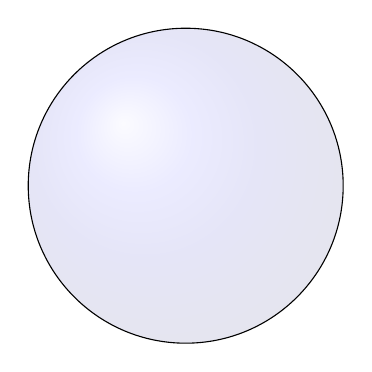
\begin{tikzpicture}
    \shade[fill opacity=0.1 ,ball color=blue] (0,0) circle (2cm);
    \draw (0,0) circle (2cm);
\end{tikzpicture}











\end{document}